\documentclass[twoside]{book}

% Packages required by doxygen
\usepackage{calc}
\usepackage{doxygen}
\usepackage{graphicx}
\usepackage[utf8]{inputenc}
\usepackage{makeidx}
\usepackage{multicol}
\usepackage{multirow}
\usepackage{textcomp}
\usepackage[table]{xcolor}

% Font selection
\usepackage[T1]{fontenc}
\usepackage{mathptmx}
\usepackage[scaled=.90]{helvet}
\usepackage{courier}
\usepackage{amssymb}
\usepackage{sectsty}
\renewcommand{\familydefault}{\sfdefault}
\allsectionsfont{%
  \fontseries{bc}\selectfont%
  \color{darkgray}%
}
\renewcommand{\DoxyLabelFont}{%
  \fontseries{bc}\selectfont%
  \color{darkgray}%
}

% Page & text layout
\usepackage{geometry}
\geometry{%
  a4paper,%
  top=2.5cm,%
  bottom=2.5cm,%
  left=2.5cm,%
  right=2.5cm%
}
\tolerance=750
\hfuzz=15pt
\hbadness=750
\setlength{\emergencystretch}{15pt}
\setlength{\parindent}{0cm}
\setlength{\parskip}{0.2cm}
\makeatletter
\renewcommand{\paragraph}{%
  \@startsection{paragraph}{4}{0ex}{-1.0ex}{1.0ex}{%
    \normalfont\normalsize\bfseries\SS@parafont%
  }%
}
\renewcommand{\subparagraph}{%
  \@startsection{subparagraph}{5}{0ex}{-1.0ex}{1.0ex}{%
    \normalfont\normalsize\bfseries\SS@subparafont%
  }%
}
\makeatother

% Headers & footers
\usepackage{fancyhdr}
\pagestyle{fancyplain}
\fancyhead[LE]{\fancyplain{}{\bfseries\thepage}}
\fancyhead[CE]{\fancyplain{}{}}
\fancyhead[RE]{\fancyplain{}{\bfseries\leftmark}}
\fancyhead[LO]{\fancyplain{}{\bfseries\rightmark}}
\fancyhead[CO]{\fancyplain{}{}}
\fancyhead[RO]{\fancyplain{}{\bfseries\thepage}}
\fancyfoot[LE]{\fancyplain{}{}}
\fancyfoot[CE]{\fancyplain{}{}}
\fancyfoot[RE]{\fancyplain{}{\bfseries\scriptsize Generated on Mon Oct 19 2015 05\-:07\-:28 for Box2\-D Main Project by Doxygen }}
\fancyfoot[LO]{\fancyplain{}{\bfseries\scriptsize Generated on Mon Oct 19 2015 05\-:07\-:28 for Box2\-D Main Project by Doxygen }}
\fancyfoot[CO]{\fancyplain{}{}}
\fancyfoot[RO]{\fancyplain{}{}}
\renewcommand{\footrulewidth}{0.4pt}
\renewcommand{\chaptermark}[1]{%
  \markboth{#1}{}%
}
\renewcommand{\sectionmark}[1]{%
  \markright{\thesection\ #1}%
}

% Indices & bibliography
\usepackage{natbib}
\usepackage[titles]{tocloft}
\setcounter{tocdepth}{3}
\setcounter{secnumdepth}{5}
\makeindex

% Hyperlinks (required, but should be loaded last)
\usepackage{ifpdf}
\ifpdf
  \usepackage[pdftex,pagebackref=true]{hyperref}
\else
  \usepackage[ps2pdf,pagebackref=true]{hyperref}
\fi
\hypersetup{%
  colorlinks=true,%
  linkcolor=blue,%
  citecolor=blue,%
  unicode%
}

% Custom commands
\newcommand{\clearemptydoublepage}{%
  \newpage{\pagestyle{empty}\cleardoublepage}%
}


%===== C O N T E N T S =====

\begin{document}

% Titlepage & ToC
\hypersetup{pageanchor=false}
\pagenumbering{roman}
\begin{titlepage}
\vspace*{7cm}
\begin{center}%
{\Large Box2\-D Main Project }\\
\vspace*{1cm}
{\large Generated by Doxygen 1.8.6}\\
\vspace*{0.5cm}
{\small Mon Oct 19 2015 05:07:28}\\
\end{center}
\end{titlepage}
\clearemptydoublepage
\tableofcontents
\clearemptydoublepage
\pagenumbering{arabic}
\hypersetup{pageanchor=true}

%--- Begin generated contents ---
\chapter{Hierarchical Index}
\section{Class Hierarchy}
This inheritance list is sorted roughly, but not completely, alphabetically\-:\begin{DoxyCompactList}
\item \contentsline{section}{Arrow}{\pageref{classArrow}}{}
\item b2\-Contact\-Listener\begin{DoxyCompactList}
\item \contentsline{section}{Test}{\pageref{classTest}}{}
\begin{DoxyCompactList}
\item \contentsline{section}{Dominos}{\pageref{classDominos}}{}
\end{DoxyCompactList}
\end{DoxyCompactList}
\item b2\-Destruction\-Listener\begin{DoxyCompactList}
\item \contentsline{section}{Destruction\-Listener}{\pageref{classDestructionListener}}{}
\end{DoxyCompactList}
\item b2\-Draw\begin{DoxyCompactList}
\item \contentsline{section}{Debug\-Draw}{\pageref{classDebugDraw}}{}
\end{DoxyCompactList}
\item b2\-Query\-Callback\begin{DoxyCompactList}
\item \contentsline{section}{Query\-Callback}{\pageref{classQueryCallback}}{}
\item \contentsline{section}{Query\-Callback2}{\pageref{classQueryCallback2}}{}
\end{DoxyCompactList}
\item \contentsline{section}{Contact\-Point}{\pageref{structContactPoint}}{}
\item \contentsline{section}{Particle\-Parameter\-:\-:Definition}{\pageref{structParticleParameter_1_1Definition}}{}
\item \contentsline{section}{Emitted\-Particle\-Callback}{\pageref{classEmittedParticleCallback}}{}
\item \contentsline{section}{Fullscreen\-U\-I}{\pageref{classFullscreenUI}}{}
\item \contentsline{section}{Particle\-Parameter}{\pageref{classParticleParameter}}{}
\item \contentsline{section}{Radial\-Emitter}{\pageref{classRadialEmitter}}{}
\item \contentsline{section}{Settings}{\pageref{structSettings}}{}
\item \contentsline{section}{Test\-Entry}{\pageref{structTestEntry}}{}
\item \contentsline{section}{Particle\-Parameter\-:\-:Value}{\pageref{structParticleParameter_1_1Value}}{}
\end{DoxyCompactList}

\chapter{Class Index}
\section{Class List}
Here are the classes, structs, unions and interfaces with brief descriptions\-:\begin{DoxyCompactList}
\item\contentsline{section}{\hyperlink{classArrow}{Arrow} }{\pageref{classArrow}}{}
\item\contentsline{section}{\hyperlink{structContactPoint}{Contact\-Point} }{\pageref{structContactPoint}}{}
\item\contentsline{section}{\hyperlink{classDebugDraw}{Debug\-Draw} }{\pageref{classDebugDraw}}{}
\item\contentsline{section}{\hyperlink{structParticleParameter_1_1Definition}{Particle\-Parameter\-::\-Definition} }{\pageref{structParticleParameter_1_1Definition}}{}
\item\contentsline{section}{\hyperlink{classDestructionListener}{Destruction\-Listener} }{\pageref{classDestructionListener}}{}
\item\contentsline{section}{\hyperlink{classDominos}{Dominos} \\*Which makes all the elements in simulation }{\pageref{classDominos}}{}
\item\contentsline{section}{\hyperlink{classEmittedParticleCallback}{Emitted\-Particle\-Callback} }{\pageref{classEmittedParticleCallback}}{}
\item\contentsline{section}{\hyperlink{classFullscreenUI}{Fullscreen\-U\-I} }{\pageref{classFullscreenUI}}{}
\item\contentsline{section}{\hyperlink{classParticleParameter}{Particle\-Parameter} }{\pageref{classParticleParameter}}{}
\item\contentsline{section}{\hyperlink{classQueryCallback}{Query\-Callback} }{\pageref{classQueryCallback}}{}
\item\contentsline{section}{\hyperlink{classQueryCallback2}{Query\-Callback2} }{\pageref{classQueryCallback2}}{}
\item\contentsline{section}{\hyperlink{classRadialEmitter}{Radial\-Emitter} }{\pageref{classRadialEmitter}}{}
\item\contentsline{section}{\hyperlink{structSettings}{Settings} \\*\hyperlink{classTest}{Test} settings. Some can be controlled in the G\-U\-I }{\pageref{structSettings}}{}
\item\contentsline{section}{\hyperlink{classTest}{Test} }{\pageref{classTest}}{}
\item\contentsline{section}{\hyperlink{structTestEntry}{Test\-Entry} }{\pageref{structTestEntry}}{}
\item\contentsline{section}{\hyperlink{structParticleParameter_1_1Value}{Particle\-Parameter\-::\-Value} }{\pageref{structParticleParameter_1_1Value}}{}
\end{DoxyCompactList}

\chapter{Class Documentation}
\hypertarget{classArrow}{\section{Arrow Class Reference}
\label{classArrow}\index{Arrow@{Arrow}}
}
\subsection*{Public Types}
\begin{DoxyCompactItemize}
\item 
enum {\bfseries Angle} \{ {\bfseries e\-\_\-angle\-Right} = 0, 
{\bfseries e\-\_\-angle\-Left} = 180
 \}
\end{DoxyCompactItemize}
\subsection*{Public Member Functions}
\begin{DoxyCompactItemize}
\item 
\hypertarget{classArrow_a4b2461c938c8ac377dcad535abad12b5}{{\bfseries Arrow} (const float32 angle, const float32 scale, const b2\-Vec2 \&position, const uint32 identifier, const b2\-Vec2 $\ast$view\-Center, const b2\-Vec2 $\ast$extents)}\label{classArrow_a4b2461c938c8ac377dcad535abad12b5}

\item 
\hypertarget{classArrow_a0a9a29065f5b4a0a9b67759591439734}{uint32 {\bfseries Get\-Identifier} () const }\label{classArrow_a0a9a29065f5b4a0a9b67759591439734}

\item 
\hypertarget{classArrow_adb07f17f92d114dc444dbefc6e84f95c}{uint32 {\bfseries Hit} (const b2\-Vec2 \&position, uint32 not\-Selected\-Identifier) const }\label{classArrow_adb07f17f92d114dc444dbefc6e84f95c}

\item 
\hypertarget{classArrow_a60685846b03df80c3673d0bae78eaf9b}{void {\bfseries Draw} (const uint32 selected\-Identifier) const }\label{classArrow_a60685846b03df80c3673d0bae78eaf9b}

\item 
\hypertarget{classArrow_a276761ef539bfbacf4a8d439c91fb451}{void {\bfseries Set\-View\-Parameters} (const b2\-Vec2 $\ast$view\-Center, const b2\-Vec2 $\ast$extents)}\label{classArrow_a276761ef539bfbacf4a8d439c91fb451}

\end{DoxyCompactItemize}
\subsection*{Static Public Attributes}
\begin{DoxyCompactItemize}
\item 
\hypertarget{classArrow_ae33379f79df205a130f23ba6a6e4c35a}{static const float32 {\bfseries k\-\_\-size} = 3.\-5f}\label{classArrow_ae33379f79df205a130f23ba6a6e4c35a}

\end{DoxyCompactItemize}
\subsection*{Protected Member Functions}
\begin{DoxyCompactItemize}
\item 
\hypertarget{classArrow_a97d389c01a79a3a53492ea61781e2e58}{float32 {\bfseries Calculate\-Scale} () const }\label{classArrow_a97d389c01a79a3a53492ea61781e2e58}

\item 
\hypertarget{classArrow_ae1f8ce58937ecd59bbc5527879d6fa73}{b2\-Vec2 $\ast$ {\bfseries Calculate\-Viewport\-Position} (b2\-Vec2 $\ast$const viewport\-Position) const }\label{classArrow_ae1f8ce58937ecd59bbc5527879d6fa73}

\end{DoxyCompactItemize}
\subsection*{Static Protected Member Functions}
\begin{DoxyCompactItemize}
\item 
\hypertarget{classArrow_ab5f952709ff30a90e6d49095099eebd2}{static void {\bfseries Draw\-Arrow} (const b2\-Color \&color, const float32 angle, const float32 scale, const b2\-Vec2 \&position)}\label{classArrow_ab5f952709ff30a90e6d49095099eebd2}

\end{DoxyCompactItemize}


\subsection{Detailed Description}


Definition at line 25 of file Arrow.\-h.



The documentation for this class was generated from the following files\-:\begin{DoxyCompactItemize}
\item 
/home/surender/box2dpro/liquidfun/\-Box2\-D/\-Testbed/\-Framework/Arrow.\-h\item 
/home/surender/box2dpro/liquidfun/\-Box2\-D/\-Testbed/\-Framework/Arrow.\-cpp\end{DoxyCompactItemize}

\hypertarget{structContactPoint}{\section{Contact\-Point Struct Reference}
\label{structContactPoint}\index{Contact\-Point@{Contact\-Point}}
}
\subsection*{Public Attributes}
\begin{DoxyCompactItemize}
\item 
\hypertarget{structContactPoint_ae0abe83cac1d16a0251c00eec2fdd9a8}{b2\-Fixture $\ast$ {\bfseries fixture\-A}}\label{structContactPoint_ae0abe83cac1d16a0251c00eec2fdd9a8}

\item 
\hypertarget{structContactPoint_a79157784afc39cf079438567b32e1612}{b2\-Fixture $\ast$ {\bfseries fixture\-B}}\label{structContactPoint_a79157784afc39cf079438567b32e1612}

\item 
\hypertarget{structContactPoint_a41bc30994cbefb7c33ed08fc5196a56e}{b2\-Vec2 {\bfseries normal}}\label{structContactPoint_a41bc30994cbefb7c33ed08fc5196a56e}

\item 
\hypertarget{structContactPoint_a4fb05c387ebf7e3d0a44c7655b5dd6b5}{b2\-Vec2 {\bfseries position}}\label{structContactPoint_a4fb05c387ebf7e3d0a44c7655b5dd6b5}

\item 
\hypertarget{structContactPoint_a1b95214f8bd0f1e8ceb4a990dd1b8cc4}{b2\-Point\-State {\bfseries state}}\label{structContactPoint_a1b95214f8bd0f1e8ceb4a990dd1b8cc4}

\item 
\hypertarget{structContactPoint_adffeee3b0c76d40d2cd397c1c0398e7a}{float32 {\bfseries normal\-Impulse}}\label{structContactPoint_adffeee3b0c76d40d2cd397c1c0398e7a}

\item 
\hypertarget{structContactPoint_a6af2d880cd0089f6ff0faeaa3437c4fa}{float32 {\bfseries tangent\-Impulse}}\label{structContactPoint_a6af2d880cd0089f6ff0faeaa3437c4fa}

\item 
\hypertarget{structContactPoint_ae462a579a9346ea2ba3d9729a45aefa7}{float32 {\bfseries separation}}\label{structContactPoint_ae462a579a9346ea2ba3d9729a45aefa7}

\end{DoxyCompactItemize}


\subsection{Detailed Description}


Definition at line 141 of file Test.\-h.



The documentation for this struct was generated from the following file\-:\begin{DoxyCompactItemize}
\item 
/home/surender/box2dpro/liquidfun/\-Box2\-D/\-Testbed/\-Framework/Test.\-h\end{DoxyCompactItemize}

\hypertarget{classDebugDraw}{\section{Debug\-Draw Class Reference}
\label{classDebugDraw}\index{Debug\-Draw@{Debug\-Draw}}
}
Inheritance diagram for Debug\-Draw\-:\begin{figure}[H]
\begin{center}
\leavevmode
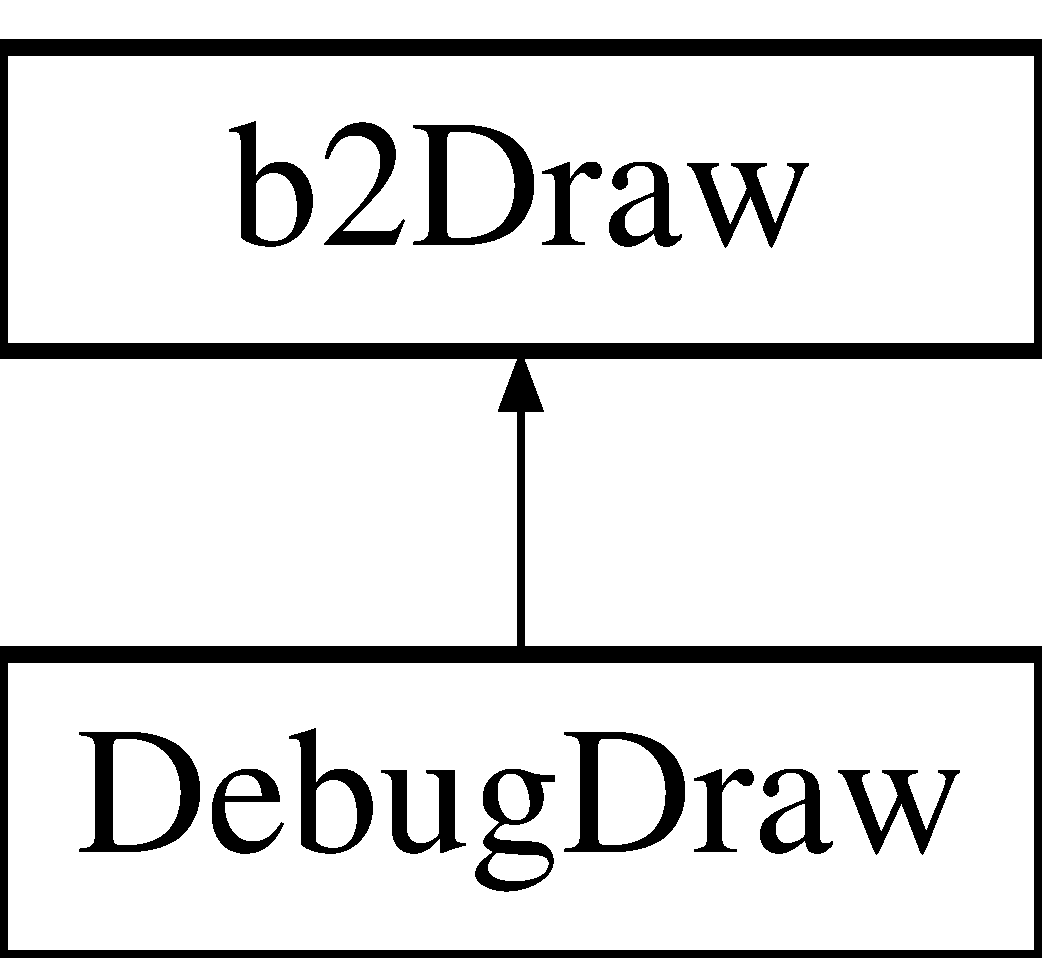
\includegraphics[height=2.000000cm]{classDebugDraw}
\end{center}
\end{figure}
\subsection*{Public Member Functions}
\begin{DoxyCompactItemize}
\item 
\hypertarget{classDebugDraw_a14ab8cf80799e57df5414db216552962}{void {\bfseries Draw\-Polygon} (const b2\-Vec2 $\ast$vertices, int32 vertex\-Count, const b2\-Color \&color)}\label{classDebugDraw_a14ab8cf80799e57df5414db216552962}

\item 
\hypertarget{classDebugDraw_a8d576ff90e7d44b220b37c18c493e55c}{void {\bfseries Draw\-Flat\-Polygon} (const b2\-Vec2 $\ast$vertices, int32 vertex\-Count, const b2\-Color \&color)}\label{classDebugDraw_a8d576ff90e7d44b220b37c18c493e55c}

\item 
\hypertarget{classDebugDraw_a1562ce91df605efef3cdf300be267cc2}{void {\bfseries Draw\-Solid\-Polygon} (const b2\-Vec2 $\ast$vertices, int32 vertex\-Count, const b2\-Color \&color)}\label{classDebugDraw_a1562ce91df605efef3cdf300be267cc2}

\item 
\hypertarget{classDebugDraw_a5adb064981a67fefe7064820006b673e}{void {\bfseries Draw\-Circle} (const b2\-Vec2 \&center, float32 radius, const b2\-Color \&color)}\label{classDebugDraw_a5adb064981a67fefe7064820006b673e}

\item 
\hypertarget{classDebugDraw_a82428519034f36a01941dd19d6108bee}{void {\bfseries Draw\-Solid\-Circle} (const b2\-Vec2 \&center, float32 radius, const b2\-Vec2 \&axis, const b2\-Color \&color)}\label{classDebugDraw_a82428519034f36a01941dd19d6108bee}

\item 
\hypertarget{classDebugDraw_a69927caae41d26f23dea336a1269ee4e}{void {\bfseries Draw\-Segment} (const b2\-Vec2 \&p1, const b2\-Vec2 \&p2, const b2\-Color \&color)}\label{classDebugDraw_a69927caae41d26f23dea336a1269ee4e}

\item 
\hypertarget{classDebugDraw_a1a12644430a648a9a683eb41e7801d21}{void {\bfseries Draw\-Particles} (const b2\-Vec2 $\ast$centers, float32 radius, const b2\-Particle\-Color $\ast$colors, int32 count)}\label{classDebugDraw_a1a12644430a648a9a683eb41e7801d21}

\item 
\hypertarget{classDebugDraw_a6f61d333e6e76865ec4a6099ab31ae75}{void {\bfseries Draw\-Transform} (const b2\-Transform \&xf)}\label{classDebugDraw_a6f61d333e6e76865ec4a6099ab31ae75}

\item 
\hypertarget{classDebugDraw_a1f9c99b818e21078a53d11a5ca6e2c79}{void {\bfseries Draw\-Point} (const b2\-Vec2 \&p, float32 size, const b2\-Color \&color)}\label{classDebugDraw_a1f9c99b818e21078a53d11a5ca6e2c79}

\item 
\hypertarget{classDebugDraw_a395164a66033cc6e3b7fb596a67f2ea4}{void {\bfseries Draw\-String} (int x, int y, const char $\ast$string,...)}\label{classDebugDraw_a395164a66033cc6e3b7fb596a67f2ea4}

\item 
\hypertarget{classDebugDraw_a906613c14254b663e714d57af5e659ee}{void {\bfseries Draw\-String} (const b2\-Vec2 \&p, const char $\ast$string,...)}\label{classDebugDraw_a906613c14254b663e714d57af5e659ee}

\item 
\hypertarget{classDebugDraw_a9a2a74e510bac791747b2b7badf750b9}{void {\bfseries Draw\-A\-A\-B\-B} (b2\-A\-A\-B\-B $\ast$aabb, const b2\-Color \&color)}\label{classDebugDraw_a9a2a74e510bac791747b2b7badf750b9}

\end{DoxyCompactItemize}


\subsection{Detailed Description}


Definition at line 36 of file Render.\-h.



The documentation for this class was generated from the following files\-:\begin{DoxyCompactItemize}
\item 
/home/surender/box2dpro/liquidfun/\-Box2\-D/\-Testbed/\-Framework/Render.\-h\item 
/home/surender/box2dpro/liquidfun/\-Box2\-D/\-Testbed/\-Framework/Render.\-cpp\end{DoxyCompactItemize}

\hypertarget{structParticleParameter_1_1Definition}{\section{Particle\-Parameter\-:\-:Definition Struct Reference}
\label{structParticleParameter_1_1Definition}\index{Particle\-Parameter\-::\-Definition@{Particle\-Parameter\-::\-Definition}}
}
\subsection*{Public Member Functions}
\begin{DoxyCompactItemize}
\item 
\hypertarget{structParticleParameter_1_1Definition_ad1bf8ccdb19046a18473da91fbd8154c}{uint32 {\bfseries Calculate\-Value\-Mask} () const }\label{structParticleParameter_1_1Definition_ad1bf8ccdb19046a18473da91fbd8154c}

\end{DoxyCompactItemize}
\subsection*{Public Attributes}
\begin{DoxyCompactItemize}
\item 
\hypertarget{structParticleParameter_1_1Definition_ac082103492ef83d6393b64249e5a51f4}{const \hyperlink{structParticleParameter_1_1Value}{Value} $\ast$ {\bfseries values}}\label{structParticleParameter_1_1Definition_ac082103492ef83d6393b64249e5a51f4}

\item 
\hypertarget{structParticleParameter_1_1Definition_ad2fe39786c3cc53652fdd9f44d3142b1}{uint32 {\bfseries num\-Values}}\label{structParticleParameter_1_1Definition_ad2fe39786c3cc53652fdd9f44d3142b1}

\end{DoxyCompactItemize}


\subsection{Detailed Description}


Definition at line 59 of file Particle\-Parameter.\-h.



The documentation for this struct was generated from the following file\-:\begin{DoxyCompactItemize}
\item 
/home/surender/box2dpro/liquidfun/\-Box2\-D/\-Testbed/\-Framework/Particle\-Parameter.\-h\end{DoxyCompactItemize}

\hypertarget{classDestructionListener}{\section{Destruction\-Listener Class Reference}
\label{classDestructionListener}\index{Destruction\-Listener@{Destruction\-Listener}}
}
Inheritance diagram for Destruction\-Listener\-:\begin{figure}[H]
\begin{center}
\leavevmode
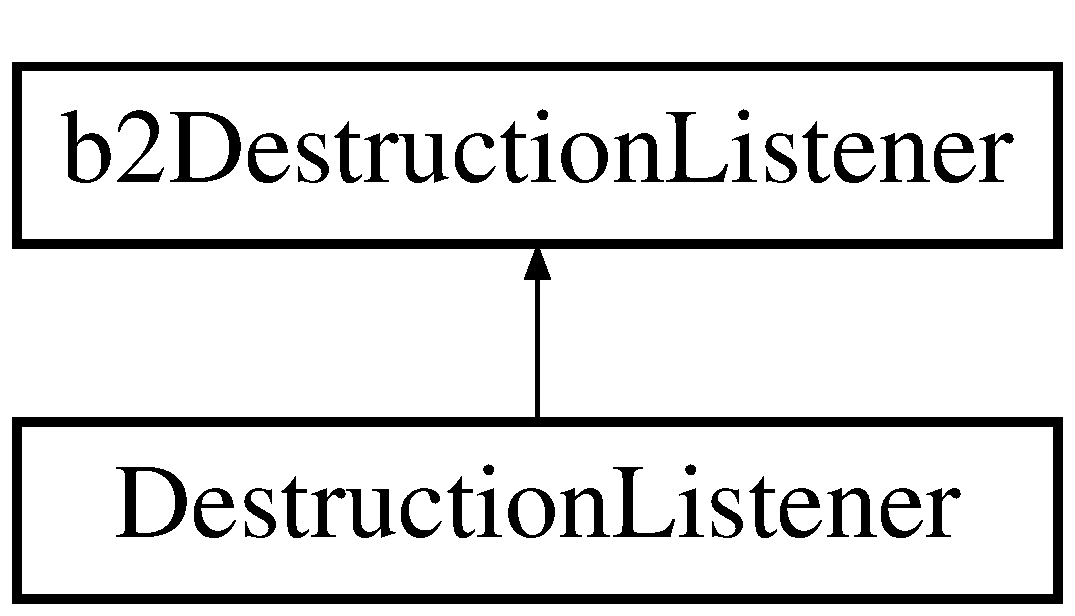
\includegraphics[height=2.000000cm]{classDestructionListener}
\end{center}
\end{figure}
\subsection*{Public Member Functions}
\begin{DoxyCompactItemize}
\item 
\hypertarget{classDestructionListener_a51b3b045b48c33fbfaa0182b329d5d49}{void {\bfseries Say\-Goodbye} (b2\-Fixture $\ast$fixture)}\label{classDestructionListener_a51b3b045b48c33fbfaa0182b329d5d49}

\item 
\hypertarget{classDestructionListener_a55627bd55b8816d66e0f3d85a75c0552}{void {\bfseries Say\-Goodbye} (b2\-Joint $\ast$joint)}\label{classDestructionListener_a55627bd55b8816d66e0f3d85a75c0552}

\item 
\hypertarget{classDestructionListener_abea64bded5c515eefa203242090d40e1}{void {\bfseries Say\-Goodbye} (b2\-Particle\-Group $\ast$group)}\label{classDestructionListener_abea64bded5c515eefa203242090d40e1}

\end{DoxyCompactItemize}
\subsection*{Public Attributes}
\begin{DoxyCompactItemize}
\item 
\hypertarget{classDestructionListener_ae6d64f92843225c30b053f942fa38402}{\hyperlink{classTest}{Test} $\ast$ {\bfseries test}}\label{classDestructionListener_ae6d64f92843225c30b053f942fa38402}

\end{DoxyCompactItemize}


\subsection{Detailed Description}


Definition at line 129 of file Test.\-h.



The documentation for this class was generated from the following files\-:\begin{DoxyCompactItemize}
\item 
/home/surender/box2dpro/liquidfun/\-Box2\-D/\-Testbed/\-Framework/Test.\-h\item 
/home/surender/box2dpro/liquidfun/\-Box2\-D/\-Testbed/\-Framework/Test.\-cpp\end{DoxyCompactItemize}

\hypertarget{classDominos}{\section{Dominos Class Reference}
\label{classDominos}\index{Dominos@{Dominos}}
}


The \hyperlink{classDominos}{Dominos} class which makes all the elements in simulation.  




{\ttfamily \#include $<$Dominos.\-h$>$}

Inheritance diagram for Dominos\-:\begin{figure}[H]
\begin{center}
\leavevmode
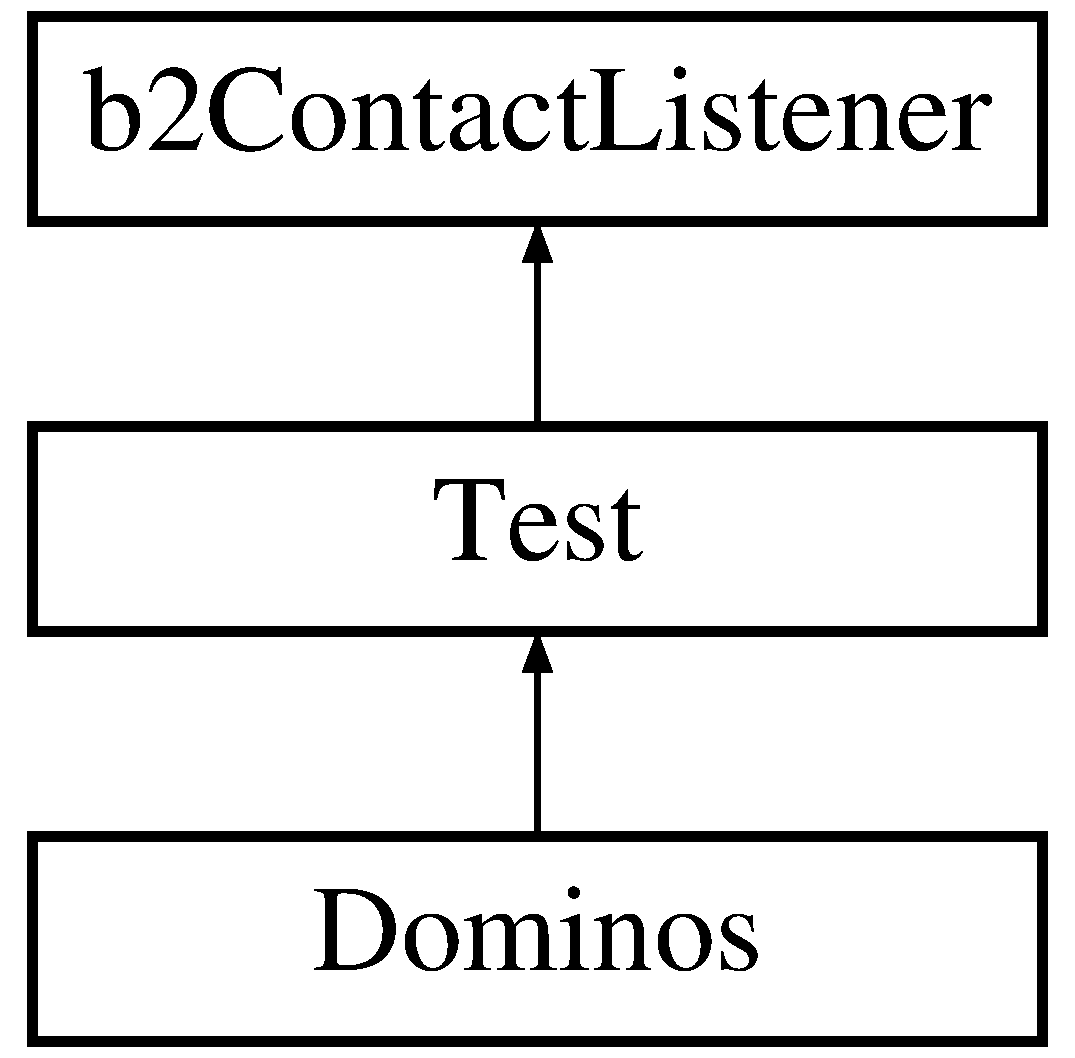
\includegraphics[height=3.000000cm]{classDominos}
\end{center}
\end{figure}
\subsection*{Public Member Functions}
\begin{DoxyCompactItemize}
\item 
\hyperlink{classDominos_a27b9b1be616966c37739fe92a38e4deb}{Dominos} ()
\item 
float32 \hyperlink{classDominos_aeb02333ccec47cebd34ec234200dd0c9}{Get\-Default\-View\-Zoom} () const 
\end{DoxyCompactItemize}
\subsection*{Static Public Member Functions}
\begin{DoxyCompactItemize}
\item 
static \hyperlink{classTest}{Test} $\ast$ \hyperlink{classDominos_a804c1c471f0eff8529a84948120f0d1a}{Create} ()
\end{DoxyCompactItemize}
\subsection*{Additional Inherited Members}


\subsection{Detailed Description}
The \hyperlink{classDominos}{Dominos} class which makes all the elements in simulation. 

It inherits \hyperlink{classTest}{Test} class and has all the code to make all the elements It has two member functions \hyperlink{classDominos_aeb02333ccec47cebd34ec234200dd0c9}{Get\-Default\-View\-Zoom()}, \hyperlink{classDominos_a804c1c471f0eff8529a84948120f0d1a}{Create()} and a constructor 

Definition at line 27 of file Dominos.\-h.



\subsection{Constructor \& Destructor Documentation}
\hypertarget{classDominos_a27b9b1be616966c37739fe92a38e4deb}{\index{Dominos@{Dominos}!Dominos@{Dominos}}
\index{Dominos@{Dominos}!Dominos@{Dominos}}
\subsubsection[{Dominos}]{\setlength{\rightskip}{0pt plus 5cm}Dominos\-::\-Dominos (
\begin{DoxyParamCaption}
{}
\end{DoxyParamCaption}
)\hspace{0.3cm}{\ttfamily [inline]}}}\label{classDominos_a27b9b1be616966c37739fe92a38e4deb}
Constructor for \hyperlink{classDominos}{Dominos} class A normal member taking no arguments and returning an float32 value representing the zoom. \begin{DoxyReturn}{Returns}
The default zoom required, Here taken as 1.\-25f 
\end{DoxyReturn}
Particles have radius set to 0.\-05f and damping to 0.\-1f

Initializing a shape 

Definition at line 34 of file Dominos.\-h.



\subsection{Member Function Documentation}
\hypertarget{classDominos_a804c1c471f0eff8529a84948120f0d1a}{\index{Dominos@{Dominos}!Create@{Create}}
\index{Create@{Create}!Dominos@{Dominos}}
\subsubsection[{Create}]{\setlength{\rightskip}{0pt plus 5cm}static {\bf Test}$\ast$ Dominos\-::\-Create (
\begin{DoxyParamCaption}
{}
\end{DoxyParamCaption}
)\hspace{0.3cm}{\ttfamily [inline]}, {\ttfamily [static]}}}\label{classDominos_a804c1c471f0eff8529a84948120f0d1a}
A normal member taking no arguments and returning an float32 value representing the zoom. \begin{DoxyReturn}{Returns}
The default zoom required, Here taken as 1.\-25f 
\end{DoxyReturn}


Definition at line 925 of file Dominos.\-h.

\hypertarget{classDominos_aeb02333ccec47cebd34ec234200dd0c9}{\index{Dominos@{Dominos}!Get\-Default\-View\-Zoom@{Get\-Default\-View\-Zoom}}
\index{Get\-Default\-View\-Zoom@{Get\-Default\-View\-Zoom}!Dominos@{Dominos}}
\subsubsection[{Get\-Default\-View\-Zoom}]{\setlength{\rightskip}{0pt plus 5cm}float32 Dominos\-::\-Get\-Default\-View\-Zoom (
\begin{DoxyParamCaption}
{}
\end{DoxyParamCaption}
) const\hspace{0.3cm}{\ttfamily [inline]}, {\ttfamily [virtual]}}}\label{classDominos_aeb02333ccec47cebd34ec234200dd0c9}
A normal member taking no arguments and returning an float32 value representing the zoom. \begin{DoxyReturn}{Returns}
The default zoom required, Here taken as 1.\-25f 
\end{DoxyReturn}


Reimplemented from \hyperlink{classTest}{Test}.



Definition at line 917 of file Dominos.\-h.



The documentation for this class was generated from the following file\-:\begin{DoxyCompactItemize}
\item 
/home/surender/box2dpro/liquidfun/\-Box2\-D/\-Testbed/\-Tests/Dominos.\-h\end{DoxyCompactItemize}

\hypertarget{classEmittedParticleCallback}{\section{Emitted\-Particle\-Callback Class Reference}
\label{classEmittedParticleCallback}\index{Emitted\-Particle\-Callback@{Emitted\-Particle\-Callback}}
}
\subsection*{Public Member Functions}
\begin{DoxyCompactItemize}
\item 
\hypertarget{classEmittedParticleCallback_a3f120672b12cbb95cb11bfd6b5ec59c2}{virtual void {\bfseries Particle\-Created} (b2\-Particle\-System $\ast$const system, const int32 particle\-Index)=0}\label{classEmittedParticleCallback_a3f120672b12cbb95cb11bfd6b5ec59c2}

\end{DoxyCompactItemize}


\subsection{Detailed Description}


Definition at line 25 of file Particle\-Emitter.\-h.



The documentation for this class was generated from the following file\-:\begin{DoxyCompactItemize}
\item 
/home/surender/box2dpro/liquidfun/\-Box2\-D/\-Testbed/\-Framework/Particle\-Emitter.\-h\end{DoxyCompactItemize}

\hypertarget{classFullscreenUI}{\section{Fullscreen\-U\-I Class Reference}
\label{classFullscreenUI}\index{Fullscreen\-U\-I@{Fullscreen\-U\-I}}
}
\subsection*{Public Types}
\begin{DoxyCompactItemize}
\item 
enum {\bfseries Selection} \{ \\*
{\bfseries e\-\_\-\-Selection\-Test\-Previous} = 0, 
{\bfseries e\-\_\-\-Selection\-Test\-Next}, 
{\bfseries e\-\_\-\-Selection\-Parameter\-Previous}, 
{\bfseries e\-\_\-\-Selection\-Parameter\-Next}, 
\\*
{\bfseries e\-\_\-\-Selection\-None}
 \}
\end{DoxyCompactItemize}
\subsection*{Public Member Functions}
\begin{DoxyCompactItemize}
\item 
\hypertarget{classFullscreenUI_a23260fc8601b7d8464ba609bc7115c1e}{void {\bfseries Reset} ()}\label{classFullscreenUI_a23260fc8601b7d8464ba609bc7115c1e}

\item 
\hypertarget{classFullscreenUI_a2096cdee1a068b504960244c4f2630c2}{bool {\bfseries Get\-Enabled} () const }\label{classFullscreenUI_a2096cdee1a068b504960244c4f2630c2}

\item 
\hypertarget{classFullscreenUI_a64c42ffa75c048a86e540362a58c6abc}{void {\bfseries Set\-Enabled} (bool enable)}\label{classFullscreenUI_a64c42ffa75c048a86e540362a58c6abc}

\item 
\hypertarget{classFullscreenUI_a4f7bc7dc03447c32338e5c47f0581793}{uint32 {\bfseries Mouse} (const int32 button, const int32 state, const int32 previous\-State, const b2\-Vec2 \&mouse\-Position)}\label{classFullscreenUI_a4f7bc7dc03447c32338e5c47f0581793}

\item 
\hypertarget{classFullscreenUI_ae8f4d06960f95c0383466e646398c142}{uint32 {\bfseries Get\-Selection} () const }\label{classFullscreenUI_ae8f4d06960f95c0383466e646398c142}

\item 
\hypertarget{classFullscreenUI_aed3f3f1e94f8b67f0bc665daa206b06a}{void {\bfseries Set\-Particle\-Parameter\-Selection\-Enabled} (const bool enable)}\label{classFullscreenUI_aed3f3f1e94f8b67f0bc665daa206b06a}

\item 
\hypertarget{classFullscreenUI_a158f8f45f150d36f6132ff10cc3b949f}{bool {\bfseries Get\-Particle\-Parameter\-Selection\-Enabled} () const }\label{classFullscreenUI_a158f8f45f150d36f6132ff10cc3b949f}

\item 
\hypertarget{classFullscreenUI_af44522cd5d4c3a3131cf013bd3daafe2}{void {\bfseries Draw} (const std\-::string \&footer)}\label{classFullscreenUI_af44522cd5d4c3a3131cf013bd3daafe2}

\item 
\hypertarget{classFullscreenUI_a03cb7469a09fe47a5f72c0202616a8f0}{void {\bfseries Set\-View\-Parameters} (const b2\-Vec2 $\ast$view\-Center, const b2\-Vec2 $\ast$extents)}\label{classFullscreenUI_a03cb7469a09fe47a5f72c0202616a8f0}

\end{DoxyCompactItemize}


\subsection{Detailed Description}


Definition at line 26 of file Fullscreen\-U\-I.\-h.



The documentation for this class was generated from the following files\-:\begin{DoxyCompactItemize}
\item 
/home/surender/box2dpro/liquidfun/\-Box2\-D/\-Testbed/\-Framework/Fullscreen\-U\-I.\-h\item 
/home/surender/box2dpro/liquidfun/\-Box2\-D/\-Testbed/\-Framework/Fullscreen\-U\-I.\-cpp\end{DoxyCompactItemize}

\hypertarget{classParticleParameter}{\section{Particle\-Parameter Class Reference}
\label{classParticleParameter}\index{Particle\-Parameter@{Particle\-Parameter}}
}
\subsection*{Classes}
\begin{DoxyCompactItemize}
\item 
struct \hyperlink{structParticleParameter_1_1Definition}{Definition}
\item 
struct \hyperlink{structParticleParameter_1_1Value}{Value}
\end{DoxyCompactItemize}
\subsection*{Public Types}
\begin{DoxyCompactItemize}
\item 
enum {\bfseries Options} \{ \\*
{\bfseries Option\-Strict\-Contacts} = 1 $<$$<$ 0, 
{\bfseries Option\-Draw\-Shapes} = 1 $<$$<$ 1, 
{\bfseries Option\-Draw\-Particles} = 1 $<$$<$ 2, 
{\bfseries Option\-Draw\-Joints} = 1 $<$$<$ 3, 
\\*
{\bfseries Option\-Draw\-A\-A\-B\-Bs} = 1 $<$$<$ 4, 
{\bfseries Option\-Draw\-Contact\-Points} = 1 $<$$<$ 5, 
{\bfseries Option\-Draw\-Contact\-Normals} = 1 $<$$<$ 6, 
{\bfseries Option\-Draw\-Contact\-Impulse} = 1 $<$$<$ 7, 
\\*
{\bfseries Option\-Draw\-Friction\-Impulse} = 1 $<$$<$ 8, 
{\bfseries Option\-Draw\-C\-O\-Ms} = 1 $<$$<$ 9, 
{\bfseries Option\-Draw\-Stats} = 1 $<$$<$ 10, 
{\bfseries Option\-Draw\-Profile} = 1 $<$$<$ 11
 \}
\end{DoxyCompactItemize}
\subsection*{Public Member Functions}
\begin{DoxyCompactItemize}
\item 
\hypertarget{classParticleParameter_ab364517111e011353969f6eb788f1a23}{void {\bfseries Reset} ()}\label{classParticleParameter_ab364517111e011353969f6eb788f1a23}

\item 
\hypertarget{classParticleParameter_a3cf2c26fae4f3f8a785ec58f482e9b1c}{void {\bfseries Set\-Definition} (const \hyperlink{structParticleParameter_1_1Definition}{Definition} $\ast$definition, uint32 definition\-Count)}\label{classParticleParameter_a3cf2c26fae4f3f8a785ec58f482e9b1c}

\item 
\hypertarget{classParticleParameter_a6521c78d03d49ddd7e991b6a28a505fc}{uint32 {\bfseries Get} () const }\label{classParticleParameter_a6521c78d03d49ddd7e991b6a28a505fc}

\item 
\hypertarget{classParticleParameter_a89d8370d708af000e429cbd761c713b9}{void {\bfseries Set} (uint32 index)}\label{classParticleParameter_a89d8370d708af000e429cbd761c713b9}

\item 
\hypertarget{classParticleParameter_ae4af7a60b490d80fcd28f4a571673e74}{void {\bfseries Increment} ()}\label{classParticleParameter_ae4af7a60b490d80fcd28f4a571673e74}

\item 
\hypertarget{classParticleParameter_ac9403cb9f9fd39f91e1c2d7264721974}{void {\bfseries Decrement} ()}\label{classParticleParameter_ac9403cb9f9fd39f91e1c2d7264721974}

\item 
\hypertarget{classParticleParameter_a837284864c63aa38ef73a31a669df4a3}{bool {\bfseries Changed} (bool $\ast$const restart)}\label{classParticleParameter_a837284864c63aa38ef73a31a669df4a3}

\item 
\hypertarget{classParticleParameter_a8e3746f690993644badb9b9bf6b11585}{uint32 {\bfseries Get\-Value} () const }\label{classParticleParameter_a8e3746f690993644badb9b9bf6b11585}

\item 
\hypertarget{classParticleParameter_aba29874ea2cc5dc0f79e91e291461889}{const char $\ast$ {\bfseries Get\-Name} () const }\label{classParticleParameter_aba29874ea2cc5dc0f79e91e291461889}

\item 
\hypertarget{classParticleParameter_aa3b19b5082fc80cd5808a65f08b1eb07}{uint32 {\bfseries Get\-Options} () const }\label{classParticleParameter_aa3b19b5082fc80cd5808a65f08b1eb07}

\item 
\hypertarget{classParticleParameter_a05cfd47650aa0293d51b98ea6a0017e1}{void {\bfseries Set\-Restart\-On\-Change} (bool enable)}\label{classParticleParameter_a05cfd47650aa0293d51b98ea6a0017e1}

\item 
\hypertarget{classParticleParameter_a5f7f827051bf973f068b3024f3ca5183}{bool {\bfseries Get\-Restart\-On\-Change} () const }\label{classParticleParameter_a5f7f827051bf973f068b3024f3ca5183}

\item 
\hypertarget{classParticleParameter_a64183933049beec1f773e433c68f84eb}{int32 {\bfseries Find\-Index\-By\-Value} (uint32 value) const }\label{classParticleParameter_a64183933049beec1f773e433c68f84eb}

\end{DoxyCompactItemize}
\subsection*{Static Public Attributes}
\begin{DoxyCompactItemize}
\item 
static const uint32 {\bfseries k\-\_\-\-Default\-Options}
\item 
static const \hyperlink{structParticleParameter_1_1Value}{Value} $\ast$ {\bfseries k\-\_\-particle\-Types\-Ptr}
\item 
static const uint32 {\bfseries k\-\_\-particle\-Types\-Count}
\item 
static const \hyperlink{structParticleParameter_1_1Value}{Value} {\bfseries k\-\_\-particle\-Types} \mbox{[}$\,$\mbox{]}
\item 
static const \hyperlink{structParticleParameter_1_1Definition}{Definition} {\bfseries k\-\_\-default\-Definition} \mbox{[}$\,$\mbox{]}
\end{DoxyCompactItemize}
\subsection*{Protected Member Functions}
\begin{DoxyCompactItemize}
\item 
\hypertarget{classParticleParameter_a5366d1aa68281e5b7ff2460234cbe218}{const \hyperlink{structParticleParameter_1_1Value}{Value} $\ast$ {\bfseries Find\-Particle\-Parameter\-Value} () const }\label{classParticleParameter_a5366d1aa68281e5b7ff2460234cbe218}

\end{DoxyCompactItemize}


\subsection{Detailed Description}


Definition at line 24 of file Particle\-Parameter.\-h.



\subsection{Member Data Documentation}
\hypertarget{classParticleParameter_a776962c86534907e7448b3f85a6e802c}{\index{Particle\-Parameter@{Particle\-Parameter}!k\-\_\-default\-Definition@{k\-\_\-default\-Definition}}
\index{k\-\_\-default\-Definition@{k\-\_\-default\-Definition}!ParticleParameter@{Particle\-Parameter}}
\subsubsection[{k\-\_\-default\-Definition}]{\setlength{\rightskip}{0pt plus 5cm}const {\bf Particle\-Parameter\-::\-Definition} Particle\-Parameter\-::k\-\_\-default\-Definition\hspace{0.3cm}{\ttfamily [static]}}}\label{classParticleParameter_a776962c86534907e7448b3f85a6e802c}
{\bfseries Initial value\-:}
\begin{DoxyCode}
=
\{
    \{
        ParticleParameter::k\_particleTypes,
        ParticleParameter::k\_particleTypesCount
    \},
\}
\end{DoxyCode}


Definition at line 165 of file Particle\-Parameter.\-h.

\hypertarget{classParticleParameter_adb8019844d1cfbec2b7eff0e1fd39bc5}{\index{Particle\-Parameter@{Particle\-Parameter}!k\-\_\-\-Default\-Options@{k\-\_\-\-Default\-Options}}
\index{k\-\_\-\-Default\-Options@{k\-\_\-\-Default\-Options}!ParticleParameter@{Particle\-Parameter}}
\subsubsection[{k\-\_\-\-Default\-Options}]{\setlength{\rightskip}{0pt plus 5cm}const uint32 Particle\-Parameter\-::k\-\_\-\-Default\-Options\hspace{0.3cm}{\ttfamily [static]}}}\label{classParticleParameter_adb8019844d1cfbec2b7eff0e1fd39bc5}
{\bfseries Initial value\-:}
\begin{DoxyCode}
=
    OptionDrawShapes | OptionDrawParticles
\end{DoxyCode}


Definition at line 44 of file Particle\-Parameter.\-h.

\hypertarget{classParticleParameter_a9be397f33beb13283cb2f1fe469c62d6}{\index{Particle\-Parameter@{Particle\-Parameter}!k\-\_\-particle\-Types@{k\-\_\-particle\-Types}}
\index{k\-\_\-particle\-Types@{k\-\_\-particle\-Types}!ParticleParameter@{Particle\-Parameter}}
\subsubsection[{k\-\_\-particle\-Types}]{\setlength{\rightskip}{0pt plus 5cm}const {\bf Particle\-Parameter\-::\-Value} Particle\-Parameter\-::k\-\_\-particle\-Types\hspace{0.3cm}{\ttfamily [static]}}}\label{classParticleParameter_a9be397f33beb13283cb2f1fe469c62d6}
{\bfseries Initial value\-:}
\begin{DoxyCode}
=
\{
    \{ b2\_waterParticle, ParticleParameter::k\_DefaultOptions, \textcolor{stringliteral}{"water"} \},
    \{ b2\_waterParticle, ParticleParameter::k\_DefaultOptions |
                ParticleParameter::OptionStrictContacts, \textcolor{stringliteral}{"water (strict)"} \},
    \{ b2\_springParticle, ParticleParameter::k\_DefaultOptions, \textcolor{stringliteral}{"spring"} \},
    \{ b2\_elasticParticle, ParticleParameter::k\_DefaultOptions, \textcolor{stringliteral}{"elastic"} \},
    \{ b2\_viscousParticle, ParticleParameter::k\_DefaultOptions, \textcolor{stringliteral}{"viscous"} \},
    \{ b2\_powderParticle, ParticleParameter::k\_DefaultOptions, \textcolor{stringliteral}{"powder"} \},
    \{ b2\_tensileParticle, ParticleParameter::k\_DefaultOptions, \textcolor{stringliteral}{"tensile"} \},
    \{ b2\_colorMixingParticle, ParticleParameter::k\_DefaultOptions,
        \textcolor{stringliteral}{"color mixing"} \},
    \{ b2\_wallParticle, ParticleParameter::k\_DefaultOptions, \textcolor{stringliteral}{"wall"} \},
    \{ b2\_barrierParticle | b2\_wallParticle,
        ParticleParameter::k\_DefaultOptions, \textcolor{stringliteral}{"barrier"} \},
    \{ b2\_staticPressureParticle, ParticleParameter::k\_DefaultOptions,
        \textcolor{stringliteral}{"static pressure"} \},
    \{ b2\_waterParticle, ParticleParameter::k\_DefaultOptions |
                ParticleParameter::OptionDrawAABBs, \textcolor{stringliteral}{"water (bounding boxes)"} \},
\}
\end{DoxyCode}


Definition at line 163 of file Particle\-Parameter.\-h.

\hypertarget{classParticleParameter_aa311f7df22a956a5f426dbae10ee98f2}{\index{Particle\-Parameter@{Particle\-Parameter}!k\-\_\-particle\-Types\-Count@{k\-\_\-particle\-Types\-Count}}
\index{k\-\_\-particle\-Types\-Count@{k\-\_\-particle\-Types\-Count}!ParticleParameter@{Particle\-Parameter}}
\subsubsection[{k\-\_\-particle\-Types\-Count}]{\setlength{\rightskip}{0pt plus 5cm}const uint32 Particle\-Parameter\-::k\-\_\-particle\-Types\-Count\hspace{0.3cm}{\ttfamily [static]}}}\label{classParticleParameter_aa311f7df22a956a5f426dbae10ee98f2}
{\bfseries Initial value\-:}
\begin{DoxyCode}
=
    B2\_ARRAY\_SIZE(ParticleParameter::k\_particleTypes)
\end{DoxyCode}


Definition at line 161 of file Particle\-Parameter.\-h.

\hypertarget{classParticleParameter_a36233222cea81fb18d1b8c530f9d75ad}{\index{Particle\-Parameter@{Particle\-Parameter}!k\-\_\-particle\-Types\-Ptr@{k\-\_\-particle\-Types\-Ptr}}
\index{k\-\_\-particle\-Types\-Ptr@{k\-\_\-particle\-Types\-Ptr}!ParticleParameter@{Particle\-Parameter}}
\subsubsection[{k\-\_\-particle\-Types\-Ptr}]{\setlength{\rightskip}{0pt plus 5cm}const {\bf Particle\-Parameter\-::\-Value} $\ast$ Particle\-Parameter\-::k\-\_\-particle\-Types\-Ptr\hspace{0.3cm}{\ttfamily [static]}}}\label{classParticleParameter_a36233222cea81fb18d1b8c530f9d75ad}
{\bfseries Initial value\-:}
\begin{DoxyCode}
=
    ParticleParameter::k\_particleTypes
\end{DoxyCode}


Definition at line 159 of file Particle\-Parameter.\-h.



The documentation for this class was generated from the following files\-:\begin{DoxyCompactItemize}
\item 
/home/surender/box2dpro/liquidfun/\-Box2\-D/\-Testbed/\-Framework/Particle\-Parameter.\-h\item 
/home/surender/box2dpro/liquidfun/\-Box2\-D/\-Testbed/\-Framework/Particle\-Parameter.\-cpp\end{DoxyCompactItemize}

\hypertarget{classQueryCallback}{\section{Query\-Callback Class Reference}
\label{classQueryCallback}\index{Query\-Callback@{Query\-Callback}}
}
Inheritance diagram for Query\-Callback\-:\begin{figure}[H]
\begin{center}
\leavevmode
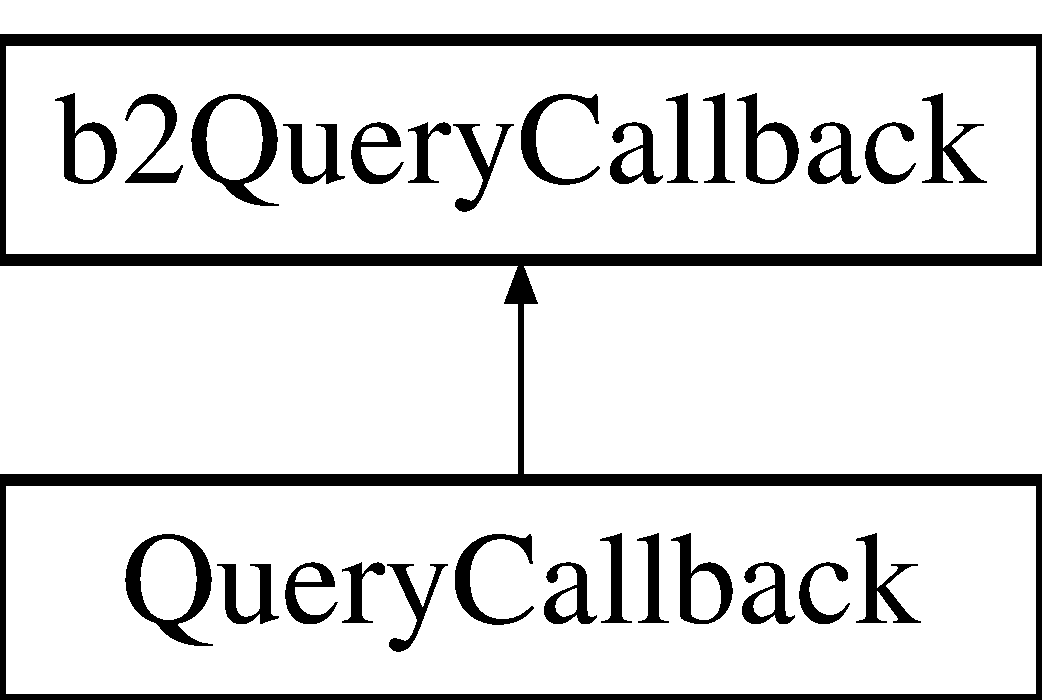
\includegraphics[height=2.000000cm]{classQueryCallback}
\end{center}
\end{figure}
\subsection*{Public Member Functions}
\begin{DoxyCompactItemize}
\item 
\hypertarget{classQueryCallback_a9c15d04aa8895b319f93e6c9af1c59f6}{{\bfseries Query\-Callback} (const b2\-Vec2 \&point)}\label{classQueryCallback_a9c15d04aa8895b319f93e6c9af1c59f6}

\item 
\hypertarget{classQueryCallback_ac79cf9e2008bdea68ab3d9d64811dc62}{bool {\bfseries Report\-Fixture} (b2\-Fixture $\ast$fixture)}\label{classQueryCallback_ac79cf9e2008bdea68ab3d9d64811dc62}

\end{DoxyCompactItemize}
\subsection*{Public Attributes}
\begin{DoxyCompactItemize}
\item 
\hypertarget{classQueryCallback_a40f98612c1a6d7eeb57a3451b4898cda}{b2\-Vec2 {\bfseries m\-\_\-point}}\label{classQueryCallback_a40f98612c1a6d7eeb57a3451b4898cda}

\item 
\hypertarget{classQueryCallback_acf7997f35f4f35b82a2aa6a9b3bd66db}{b2\-Fixture $\ast$ {\bfseries m\-\_\-fixture}}\label{classQueryCallback_acf7997f35f4f35b82a2aa6a9b3bd66db}

\end{DoxyCompactItemize}


\subsection{Detailed Description}


Definition at line 142 of file Test.\-cpp.



The documentation for this class was generated from the following file\-:\begin{DoxyCompactItemize}
\item 
/home/surender/box2dpro/liquidfun/\-Box2\-D/\-Testbed/\-Framework/Test.\-cpp\end{DoxyCompactItemize}

\hypertarget{classQueryCallback2}{\section{Query\-Callback2 Class Reference}
\label{classQueryCallback2}\index{Query\-Callback2@{Query\-Callback2}}
}
Inheritance diagram for Query\-Callback2\-:\begin{figure}[H]
\begin{center}
\leavevmode
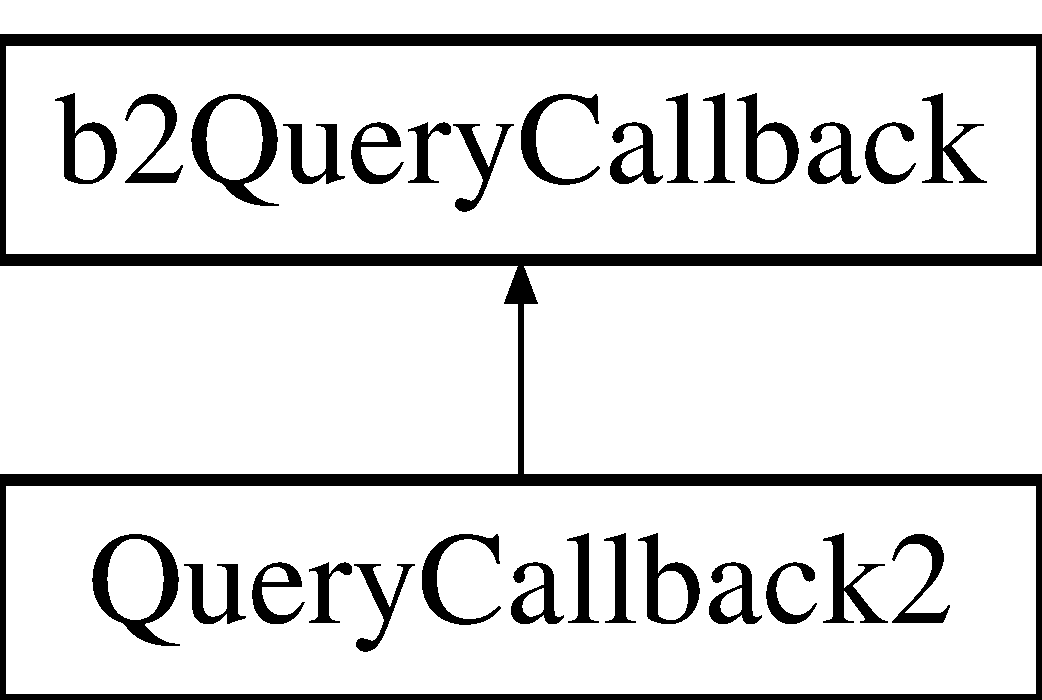
\includegraphics[height=2.000000cm]{classQueryCallback2}
\end{center}
\end{figure}
\subsection*{Public Member Functions}
\begin{DoxyCompactItemize}
\item 
\hypertarget{classQueryCallback2_a02424794d93face18cb282124788ce50}{{\bfseries Query\-Callback2} (b2\-Particle\-System $\ast$particle\-System, const b2\-Shape $\ast$shape, const b2\-Vec2 \&velocity)}\label{classQueryCallback2_a02424794d93face18cb282124788ce50}

\item 
\hypertarget{classQueryCallback2_addabdd594fa18ef09a03ec292417e2f6}{bool {\bfseries Report\-Fixture} (b2\-Fixture $\ast$fixture)}\label{classQueryCallback2_addabdd594fa18ef09a03ec292417e2f6}

\item 
\hypertarget{classQueryCallback2_a328cfeed630549c310dd94ed2bd85908}{bool {\bfseries Report\-Particle} (const b2\-Particle\-System $\ast$particle\-System, int32 index)}\label{classQueryCallback2_a328cfeed630549c310dd94ed2bd85908}

\end{DoxyCompactItemize}
\subsection*{Public Attributes}
\begin{DoxyCompactItemize}
\item 
\hypertarget{classQueryCallback2_adaf7d6830942d6eb9f833a941fabdddb}{b2\-Particle\-System $\ast$ {\bfseries m\-\_\-particle\-System}}\label{classQueryCallback2_adaf7d6830942d6eb9f833a941fabdddb}

\item 
\hypertarget{classQueryCallback2_a6f9b622a9bf8875190c8da9fcac340fd}{const b2\-Shape $\ast$ {\bfseries m\-\_\-shape}}\label{classQueryCallback2_a6f9b622a9bf8875190c8da9fcac340fd}

\item 
\hypertarget{classQueryCallback2_a5d345f512492fcdec190ec87afd69e0c}{b2\-Vec2 {\bfseries m\-\_\-velocity}}\label{classQueryCallback2_a5d345f512492fcdec190ec87afd69e0c}

\end{DoxyCompactItemize}


\subsection{Detailed Description}


Definition at line 174 of file Test.\-cpp.



The documentation for this class was generated from the following file\-:\begin{DoxyCompactItemize}
\item 
/home/surender/box2dpro/liquidfun/\-Box2\-D/\-Testbed/\-Framework/Test.\-cpp\end{DoxyCompactItemize}

\hypertarget{classRadialEmitter}{\section{Radial\-Emitter Class Reference}
\label{classRadialEmitter}\index{Radial\-Emitter@{Radial\-Emitter}}
}
\subsection*{Public Member Functions}
\begin{DoxyCompactItemize}
\item 
\hypertarget{classRadialEmitter_ad6cd678da500e22790b3a2dc374e8549}{void {\bfseries Set\-Position} (const b2\-Vec2 \&origin)}\label{classRadialEmitter_ad6cd678da500e22790b3a2dc374e8549}

\item 
\hypertarget{classRadialEmitter_aeb1d185225b71e127da95932bf910dd8}{const b2\-Vec2 \& {\bfseries Get\-Position} () const }\label{classRadialEmitter_aeb1d185225b71e127da95932bf910dd8}

\item 
\hypertarget{classRadialEmitter_a3b124352b3aad592e8054fa9218c48f5}{void {\bfseries Set\-Size} (const b2\-Vec2 \&size)}\label{classRadialEmitter_a3b124352b3aad592e8054fa9218c48f5}

\item 
\hypertarget{classRadialEmitter_a959615606bd366b01026653e9fe6763e}{b2\-Vec2 {\bfseries Get\-Size} () const }\label{classRadialEmitter_a959615606bd366b01026653e9fe6763e}

\item 
\hypertarget{classRadialEmitter_acc1d88a4901decedaace742b771502d4}{void {\bfseries Set\-Velocity} (const b2\-Vec2 \&velocity)}\label{classRadialEmitter_acc1d88a4901decedaace742b771502d4}

\item 
\hypertarget{classRadialEmitter_a37f646c0d0f0d31ef8859f971d48dcfe}{const b2\-Vec2 \& {\bfseries Get\-Velocity} () const }\label{classRadialEmitter_a37f646c0d0f0d31ef8859f971d48dcfe}

\item 
\hypertarget{classRadialEmitter_aaad20e59d0c686e5154e02e43a41e8ff}{void {\bfseries Set\-Speed} (const float32 speed)}\label{classRadialEmitter_aaad20e59d0c686e5154e02e43a41e8ff}

\item 
\hypertarget{classRadialEmitter_a37b9cec093f04dcdc63134dbeedbcf03}{float32 {\bfseries Get\-Speed} () const }\label{classRadialEmitter_a37b9cec093f04dcdc63134dbeedbcf03}

\item 
\hypertarget{classRadialEmitter_af397a1f783787fea82d0a3196090e4bf}{void {\bfseries Set\-Particle\-Flags} (uint32 flags)}\label{classRadialEmitter_af397a1f783787fea82d0a3196090e4bf}

\item 
\hypertarget{classRadialEmitter_aca340fca74f54c4f37a697011ac60f94}{uint32 {\bfseries Get\-Particle\-Flags} () const }\label{classRadialEmitter_aca340fca74f54c4f37a697011ac60f94}

\item 
\hypertarget{classRadialEmitter_af88a107b46d81953d5ee1fa0f9a0db33}{void {\bfseries Set\-Color} (const b2\-Particle\-Color \&color)}\label{classRadialEmitter_af88a107b46d81953d5ee1fa0f9a0db33}

\item 
\hypertarget{classRadialEmitter_a4076754f3619abf5bfba7ab121cb3369}{const b2\-Particle\-Color \& {\bfseries Get\-Color} () const }\label{classRadialEmitter_a4076754f3619abf5bfba7ab121cb3369}

\item 
\hypertarget{classRadialEmitter_a9ef46fd5e52e3e81f73594db90019e2c}{void {\bfseries Set\-Emit\-Rate} (const float32 emit\-Rate)}\label{classRadialEmitter_a9ef46fd5e52e3e81f73594db90019e2c}

\item 
\hypertarget{classRadialEmitter_a8f2ed81d05d5ecbc74084dc7b6d1ba9b}{float32 {\bfseries Get\-Emit\-Rate} () const }\label{classRadialEmitter_a8f2ed81d05d5ecbc74084dc7b6d1ba9b}

\item 
\hypertarget{classRadialEmitter_a3ebdd4139fffc06d4c96cfff99eccf8c}{void {\bfseries Set\-Particle\-System} (b2\-Particle\-System $\ast$const particle\-System)}\label{classRadialEmitter_a3ebdd4139fffc06d4c96cfff99eccf8c}

\item 
\hypertarget{classRadialEmitter_a094b585f881dde7f20b139ef26ea041d}{b2\-Particle\-System $\ast$ {\bfseries Get\-Particle\-System} () const }\label{classRadialEmitter_a094b585f881dde7f20b139ef26ea041d}

\item 
\hypertarget{classRadialEmitter_af1e48268753129d0996cc67a7be664aa}{void {\bfseries Set\-Callback} (\hyperlink{classEmittedParticleCallback}{Emitted\-Particle\-Callback} $\ast$const callback)}\label{classRadialEmitter_af1e48268753129d0996cc67a7be664aa}

\item 
\hypertarget{classRadialEmitter_acf08ecb75ff414cf648cb7d0992021d4}{\hyperlink{classEmittedParticleCallback}{Emitted\-Particle\-Callback} $\ast$ {\bfseries Get\-Callback} () const }\label{classRadialEmitter_acf08ecb75ff414cf648cb7d0992021d4}

\item 
\hypertarget{classRadialEmitter_acbb9e0c18921b08cd37ed17e569aae57}{void {\bfseries Set\-Group} (b2\-Particle\-Group $\ast$const group)}\label{classRadialEmitter_acbb9e0c18921b08cd37ed17e569aae57}

\item 
\hypertarget{classRadialEmitter_a089212502b68ff0d67c0a1e5fc2167e9}{b2\-Particle\-Group $\ast$ {\bfseries Get\-Group} () const }\label{classRadialEmitter_a089212502b68ff0d67c0a1e5fc2167e9}

\item 
\hypertarget{classRadialEmitter_a66bf43ec3f1454127cf2a02de08f523c}{int32 {\bfseries Step} (const float32 dt, int32 $\ast$const particle\-Indices, const int32 particle\-Indices\-Count)}\label{classRadialEmitter_a66bf43ec3f1454127cf2a02de08f523c}

\end{DoxyCompactItemize}


\subsection{Detailed Description}


Definition at line 36 of file Particle\-Emitter.\-h.



The documentation for this class was generated from the following file\-:\begin{DoxyCompactItemize}
\item 
/home/surender/box2dpro/liquidfun/\-Box2\-D/\-Testbed/\-Framework/Particle\-Emitter.\-h\end{DoxyCompactItemize}

\hypertarget{structSettings}{\section{Settings Struct Reference}
\label{structSettings}\index{Settings@{Settings}}
}


\hyperlink{classTest}{Test} settings. Some can be controlled in the G\-U\-I.  




{\ttfamily \#include $<$Test.\-h$>$}

\subsection*{Public Attributes}
\begin{DoxyCompactItemize}
\item 
\hypertarget{structSettings_a9f73ff7bfe24c0ec00f00637ad660afa}{b2\-Vec2 {\bfseries view\-Center}}\label{structSettings_a9f73ff7bfe24c0ec00f00637ad660afa}

\item 
\hypertarget{structSettings_a81f52938e3bfe4976755e77e940ca0e0}{float32 {\bfseries hz}}\label{structSettings_a81f52938e3bfe4976755e77e940ca0e0}

\item 
\hypertarget{structSettings_aef56168e9043d5a6f264a57fc0d0823a}{int32 {\bfseries velocity\-Iterations}}\label{structSettings_aef56168e9043d5a6f264a57fc0d0823a}

\item 
\hypertarget{structSettings_ae66b1defd12295dd5dce2362fcdad12f}{int32 {\bfseries position\-Iterations}}\label{structSettings_ae66b1defd12295dd5dce2362fcdad12f}

\item 
\hypertarget{structSettings_ab0b9829f65998b56807ab6d30d013e56}{int32 {\bfseries particle\-Iterations}}\label{structSettings_ab0b9829f65998b56807ab6d30d013e56}

\item 
\hypertarget{structSettings_a4a8172dd21368b12a8442723f30914bf}{int32 {\bfseries draw\-Shapes}}\label{structSettings_a4a8172dd21368b12a8442723f30914bf}

\item 
\hypertarget{structSettings_a91ba62f62bb55f5332765b10e0dd9033}{int32 {\bfseries draw\-Particles}}\label{structSettings_a91ba62f62bb55f5332765b10e0dd9033}

\item 
\hypertarget{structSettings_ab03e798642ff7d039d5efa3e0d5e86cb}{int32 {\bfseries draw\-Joints}}\label{structSettings_ab03e798642ff7d039d5efa3e0d5e86cb}

\item 
\hypertarget{structSettings_a7ac6f10e3c8e20e8e9a7b7fa90f4b5b5}{int32 {\bfseries draw\-A\-A\-B\-Bs}}\label{structSettings_a7ac6f10e3c8e20e8e9a7b7fa90f4b5b5}

\item 
\hypertarget{structSettings_afdc2b5f2611fc52d082e2ff69242cd9b}{int32 {\bfseries draw\-Contact\-Points}}\label{structSettings_afdc2b5f2611fc52d082e2ff69242cd9b}

\item 
\hypertarget{structSettings_ad95473a203267e76c613f3a7c2677836}{int32 {\bfseries draw\-Contact\-Normals}}\label{structSettings_ad95473a203267e76c613f3a7c2677836}

\item 
\hypertarget{structSettings_a6fc7ce0812268ff068423e96e11e0a54}{int32 {\bfseries draw\-Contact\-Impulse}}\label{structSettings_a6fc7ce0812268ff068423e96e11e0a54}

\item 
\hypertarget{structSettings_a077d666f6ee1feaaf6a6fe033c03e157}{int32 {\bfseries draw\-Friction\-Impulse}}\label{structSettings_a077d666f6ee1feaaf6a6fe033c03e157}

\item 
\hypertarget{structSettings_af5595d1914a8f3b76b43224cc16f05fc}{int32 {\bfseries draw\-C\-O\-Ms}}\label{structSettings_af5595d1914a8f3b76b43224cc16f05fc}

\item 
\hypertarget{structSettings_ac1dc47bd42cb02ab564d16973c3ac235}{int32 {\bfseries draw\-Stats}}\label{structSettings_ac1dc47bd42cb02ab564d16973c3ac235}

\item 
\hypertarget{structSettings_ab2f2f8bbbd3cf9997000d229f4caff31}{int32 {\bfseries draw\-Profile}}\label{structSettings_ab2f2f8bbbd3cf9997000d229f4caff31}

\item 
\hypertarget{structSettings_adb8ab5ccbdefc201db87e2d451df1758}{int32 {\bfseries enable\-Warm\-Starting}}\label{structSettings_adb8ab5ccbdefc201db87e2d451df1758}

\item 
\hypertarget{structSettings_a5c4a2f9de9c8934d149dc352fc600bf1}{int32 {\bfseries enable\-Continuous}}\label{structSettings_a5c4a2f9de9c8934d149dc352fc600bf1}

\item 
\hypertarget{structSettings_a13446b165febfb28b59adcce030d29cc}{int32 {\bfseries enable\-Sub\-Stepping}}\label{structSettings_a13446b165febfb28b59adcce030d29cc}

\item 
\hypertarget{structSettings_aa78c71c9cf421a97550c4c108dc101b4}{int32 {\bfseries enable\-Sleep}}\label{structSettings_aa78c71c9cf421a97550c4c108dc101b4}

\item 
\hypertarget{structSettings_a8be95d53012a813806bd14fdf3d02885}{int32 {\bfseries pause}}\label{structSettings_a8be95d53012a813806bd14fdf3d02885}

\item 
\hypertarget{structSettings_ab26356e864848394be4ae8bc76850d05}{int32 {\bfseries single\-Step}}\label{structSettings_ab26356e864848394be4ae8bc76850d05}

\item 
\hypertarget{structSettings_a1213104d2d7e03fb9132c5728a60e0d2}{int32 {\bfseries print\-Step\-Time\-Stats}}\label{structSettings_a1213104d2d7e03fb9132c5728a60e0d2}

\item 
\hypertarget{structSettings_a92a470f22525c9eb07d1d4984460b920}{int32 {\bfseries strict\-Contacts}}\label{structSettings_a92a470f22525c9eb07d1d4984460b920}

\item 
\hypertarget{structSettings_af9f07b2174ca26b523fd1cd5aad1ad22}{float32 \hyperlink{structSettings_af9f07b2174ca26b523fd1cd5aad1ad22}{step\-Time\-Out}}\label{structSettings_af9f07b2174ca26b523fd1cd5aad1ad22}

\begin{DoxyCompactList}\small\item\em Measures how long did the world step took, in ms. \end{DoxyCompactList}\end{DoxyCompactItemize}


\subsection{Detailed Description}
\hyperlink{classTest}{Test} settings. Some can be controlled in the G\-U\-I. 

Definition at line 56 of file Test.\-h.



The documentation for this struct was generated from the following file\-:\begin{DoxyCompactItemize}
\item 
/home/surender/box2dpro/liquidfun/\-Box2\-D/\-Testbed/\-Framework/Test.\-h\end{DoxyCompactItemize}

\hypertarget{classTest}{\section{Test Class Reference}
\label{classTest}\index{Test@{Test}}
}
Inheritance diagram for Test\-:\begin{figure}[H]
\begin{center}
\leavevmode
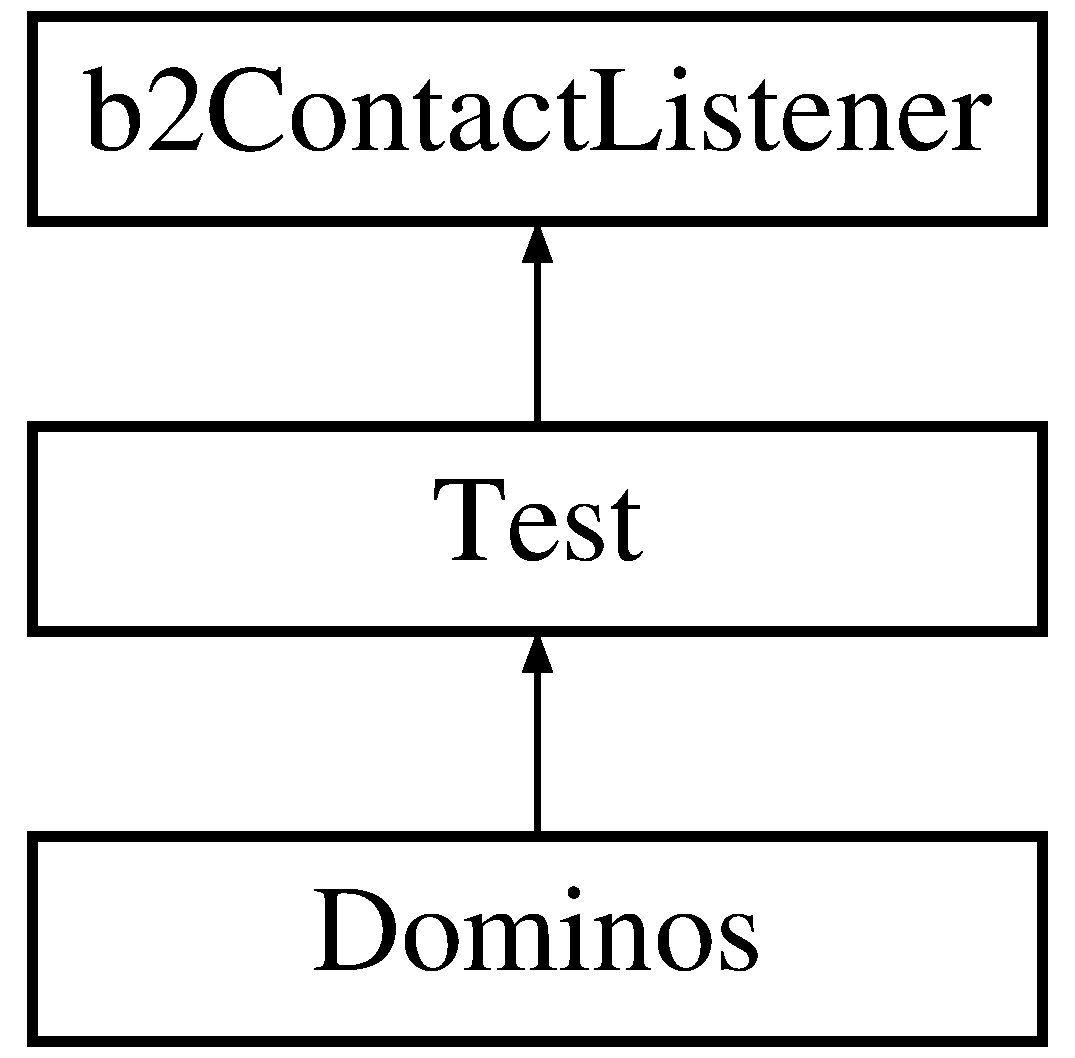
\includegraphics[height=3.000000cm]{classTest}
\end{center}
\end{figure}
\subsection*{Public Member Functions}
\begin{DoxyCompactItemize}
\item 
\hypertarget{classTest_adc34013ff19f072ebc1cff1fe8fadb51}{void {\bfseries Draw\-Title} (const char $\ast$string)}\label{classTest_adc34013ff19f072ebc1cff1fe8fadb51}

\item 
\hypertarget{classTest_af17783fea09eebb98fc500af85f2d330}{virtual void {\bfseries Step} (\hyperlink{structSettings}{Settings} $\ast$settings)}\label{classTest_af17783fea09eebb98fc500af85f2d330}

\item 
\hypertarget{classTest_a794e4d4a30c1e7f13b62eb775e59c012}{virtual void {\bfseries Keyboard} (unsigned char key)}\label{classTest_a794e4d4a30c1e7f13b62eb775e59c012}

\item 
\hypertarget{classTest_ab318e010754ba899e7fa646d6f22c1ab}{virtual void {\bfseries Keyboard\-Up} (unsigned char key)}\label{classTest_ab318e010754ba899e7fa646d6f22c1ab}

\item 
\hypertarget{classTest_aefa1d0ec080ed52b0a6b37664b6f75cd}{void {\bfseries Shift\-Mouse\-Down} (const b2\-Vec2 \&p)}\label{classTest_aefa1d0ec080ed52b0a6b37664b6f75cd}

\item 
\hypertarget{classTest_aa6382879085349085ffd17e212cfa52b}{virtual void {\bfseries Mouse\-Down} (const b2\-Vec2 \&p)}\label{classTest_aa6382879085349085ffd17e212cfa52b}

\item 
\hypertarget{classTest_a6b9adb9e42c85a5519ab31cd57063da7}{virtual void {\bfseries Mouse\-Up} (const b2\-Vec2 \&p)}\label{classTest_a6b9adb9e42c85a5519ab31cd57063da7}

\item 
\hypertarget{classTest_a043a2d8dea5248b839c501e03df97475}{virtual void {\bfseries Mouse\-Move} (const b2\-Vec2 \&p)}\label{classTest_a043a2d8dea5248b839c501e03df97475}

\item 
\hypertarget{classTest_a3f004c3be556e7765e39c59ba1561441}{void {\bfseries Launch\-Bomb} ()}\label{classTest_a3f004c3be556e7765e39c59ba1561441}

\item 
\hypertarget{classTest_a433791c82ebf92a7e9c1b35463158008}{void {\bfseries Launch\-Bomb} (const b2\-Vec2 \&position, const b2\-Vec2 \&velocity)}\label{classTest_a433791c82ebf92a7e9c1b35463158008}

\item 
\hypertarget{classTest_a3c7ac01710bbc0371aa0513b970cb4a4}{void {\bfseries Spawn\-Bomb} (const b2\-Vec2 \&world\-Pt)}\label{classTest_a3c7ac01710bbc0371aa0513b970cb4a4}

\item 
\hypertarget{classTest_a5f79351b4f312e7ecbdbfd92e76fc806}{void {\bfseries Complete\-Bomb\-Spawn} (const b2\-Vec2 \&p)}\label{classTest_a5f79351b4f312e7ecbdbfd92e76fc806}

\item 
\hypertarget{classTest_a27badb0e44400afbbbb101e58ac7bf4f}{virtual void {\bfseries Joint\-Destroyed} (b2\-Joint $\ast$joint)}\label{classTest_a27badb0e44400afbbbb101e58ac7bf4f}

\item 
\hypertarget{classTest_a6ba300758e0ee4307159d689d91d38ac}{virtual void {\bfseries Particle\-Group\-Destroyed} (b2\-Particle\-Group $\ast$group)}\label{classTest_a6ba300758e0ee4307159d689d91d38ac}

\item 
\hypertarget{classTest_ade381c3186c925cdf5dc30b0153411ba}{virtual void {\bfseries Begin\-Contact} (b2\-Contact $\ast$contact)}\label{classTest_ade381c3186c925cdf5dc30b0153411ba}

\item 
\hypertarget{classTest_a07844a975adb8d27f9523db4addd9813}{virtual void {\bfseries End\-Contact} (b2\-Contact $\ast$contact)}\label{classTest_a07844a975adb8d27f9523db4addd9813}

\item 
\hypertarget{classTest_ab815ed5d709ccbcbe567838e01fe30c4}{virtual void {\bfseries Pre\-Solve} (b2\-Contact $\ast$contact, const b2\-Manifold $\ast$old\-Manifold)}\label{classTest_ab815ed5d709ccbcbe567838e01fe30c4}

\item 
\hypertarget{classTest_a7e4aa8d83b8aa30bcd40cf9b1fde2193}{virtual void {\bfseries Post\-Solve} (b2\-Contact $\ast$contact, const b2\-Contact\-Impulse $\ast$impulse)}\label{classTest_a7e4aa8d83b8aa30bcd40cf9b1fde2193}

\item 
\hypertarget{classTest_a447e17296ea650120b44ec31f71bb12f}{void {\bfseries Shift\-Origin} (const b2\-Vec2 \&new\-Origin)}\label{classTest_a447e17296ea650120b44ec31f71bb12f}

\item 
\hypertarget{classTest_a19ff7392fd33f09ea12187c660ed329b}{virtual float32 {\bfseries Get\-Default\-View\-Zoom} () const }\label{classTest_a19ff7392fd33f09ea12187c660ed329b}

\item 
\hypertarget{classTest_a57ea3d3bcffc950d4479eaab6ad99fcd}{void {\bfseries Color\-Particle\-Group} (b2\-Particle\-Group $\ast$const group, uint32 particles\-Per\-Color)}\label{classTest_a57ea3d3bcffc950d4479eaab6ad99fcd}

\item 
\hypertarget{classTest_ab8a008ae71118b79267caa4add5d705d}{void {\bfseries Initialize\-Particle\-Parameters} (const uint32 filter\-Mask)}\label{classTest_ab8a008ae71118b79267caa4add5d705d}

\item 
\hypertarget{classTest_a2decee2179856d30e9bbe9ef39ffee41}{void {\bfseries Restore\-Particle\-Parameters} ()}\label{classTest_a2decee2179856d30e9bbe9ef39ffee41}

\end{DoxyCompactItemize}
\subsection*{Protected Attributes}
\begin{DoxyCompactItemize}
\item 
\hypertarget{classTest_af0a331a4ee6914e6abe263759c3b3705}{b2\-Body $\ast$ {\bfseries m\-\_\-ground\-Body}}\label{classTest_af0a331a4ee6914e6abe263759c3b3705}

\item 
\hypertarget{classTest_ac1c97085c255562129e6e083f1669617}{b2\-A\-A\-B\-B {\bfseries m\-\_\-world\-A\-A\-B\-B}}\label{classTest_ac1c97085c255562129e6e083f1669617}

\item 
\hypertarget{classTest_a3e8d8a7956cbb8c379e4bb917eb44f67}{\hyperlink{structContactPoint}{Contact\-Point} {\bfseries m\-\_\-points} \mbox{[}k\-\_\-max\-Contact\-Points\mbox{]}}\label{classTest_a3e8d8a7956cbb8c379e4bb917eb44f67}

\item 
\hypertarget{classTest_a1c42f2908bb7ec1a04b2d2c35c974b05}{int32 {\bfseries m\-\_\-point\-Count}}\label{classTest_a1c42f2908bb7ec1a04b2d2c35c974b05}

\item 
\hypertarget{classTest_a1d407eb8533e2c310995e60c9abdb37c}{\hyperlink{classDestructionListener}{Destruction\-Listener} {\bfseries m\-\_\-destruction\-Listener}}\label{classTest_a1d407eb8533e2c310995e60c9abdb37c}

\item 
\hypertarget{classTest_a639536a3e73f7cfa8a311559eef4d6a7}{\hyperlink{classDebugDraw}{Debug\-Draw} {\bfseries m\-\_\-debug\-Draw}}\label{classTest_a639536a3e73f7cfa8a311559eef4d6a7}

\item 
\hypertarget{classTest_a4f796421176f321ee8e82f82206c8445}{int32 {\bfseries m\-\_\-text\-Line}}\label{classTest_a4f796421176f321ee8e82f82206c8445}

\item 
\hypertarget{classTest_abadd9abd618accf5f759c4d3759c50c3}{b2\-World $\ast$ {\bfseries m\-\_\-world}}\label{classTest_abadd9abd618accf5f759c4d3759c50c3}

\item 
\hypertarget{classTest_a8217aa4a96a0856bb7f69e75ff5004ae}{b2\-Particle\-System $\ast$ {\bfseries m\-\_\-particle\-System}}\label{classTest_a8217aa4a96a0856bb7f69e75ff5004ae}

\item 
\hypertarget{classTest_a12655cb6ce6b68ce3ac6a445d2a21339}{b2\-Body $\ast$ {\bfseries m\-\_\-bomb}}\label{classTest_a12655cb6ce6b68ce3ac6a445d2a21339}

\item 
\hypertarget{classTest_a0034c1fd7c2417cf2eccb64068c2c0ea}{b2\-Mouse\-Joint $\ast$ {\bfseries m\-\_\-mouse\-Joint}}\label{classTest_a0034c1fd7c2417cf2eccb64068c2c0ea}

\item 
\hypertarget{classTest_ad2dd7ba39707588ef5f1bc27b3d5425d}{b2\-Vec2 {\bfseries m\-\_\-bomb\-Spawn\-Point}}\label{classTest_ad2dd7ba39707588ef5f1bc27b3d5425d}

\item 
\hypertarget{classTest_a27320dd554f06608058fc17c63df3aef}{bool {\bfseries m\-\_\-bomb\-Spawning}}\label{classTest_a27320dd554f06608058fc17c63df3aef}

\item 
\hypertarget{classTest_a7c7cad34d65be96e3e0b5647cb1fb0b1}{b2\-Vec2 {\bfseries m\-\_\-mouse\-World}}\label{classTest_a7c7cad34d65be96e3e0b5647cb1fb0b1}

\item 
\hypertarget{classTest_a47452fcf9cdfaeb770ff877ca1de23ba}{bool {\bfseries m\-\_\-mouse\-Tracing}}\label{classTest_a47452fcf9cdfaeb770ff877ca1de23ba}

\item 
\hypertarget{classTest_afc0307509c7619d99e06177d25b7da0c}{b2\-Vec2 {\bfseries m\-\_\-mouse\-Tracer\-Position}}\label{classTest_afc0307509c7619d99e06177d25b7da0c}

\item 
\hypertarget{classTest_a84b1e492afdaa8196a834ef1256f7ae0}{b2\-Vec2 {\bfseries m\-\_\-mouse\-Tracer\-Velocity}}\label{classTest_a84b1e492afdaa8196a834ef1256f7ae0}

\item 
\hypertarget{classTest_aeba7befe157e2897d4f4cbae18cfe87a}{int32 {\bfseries m\-\_\-step\-Count}}\label{classTest_aeba7befe157e2897d4f4cbae18cfe87a}

\item 
\hypertarget{classTest_a62c3b995fdfb0cbdfb8443c5af0147d7}{b2\-Profile {\bfseries m\-\_\-max\-Profile}}\label{classTest_a62c3b995fdfb0cbdfb8443c5af0147d7}

\item 
\hypertarget{classTest_a620017b99e7e4d2d3ff17a89faebc00b}{b2\-Profile {\bfseries m\-\_\-total\-Profile}}\label{classTest_a620017b99e7e4d2d3ff17a89faebc00b}

\item 
\hypertarget{classTest_a06702c85024baa29a49241f8da875d1c}{\hyperlink{structParticleParameter_1_1Value}{Particle\-Parameter\-::\-Value} $\ast$ {\bfseries m\-\_\-particle\-Parameters}}\label{classTest_a06702c85024baa29a49241f8da875d1c}

\item 
\hypertarget{classTest_af526852ab6e9911dc2a4ccf47401fe91}{\hyperlink{structParticleParameter_1_1Definition}{Particle\-Parameter\-::\-Definition} {\bfseries m\-\_\-particle\-Parameter\-Def}}\label{classTest_af526852ab6e9911dc2a4ccf47401fe91}

\end{DoxyCompactItemize}
\subsection*{Static Protected Attributes}
\begin{DoxyCompactItemize}
\item 
static const b2\-Particle\-Color {\bfseries k\-\_\-\-Particle\-Colors} \mbox{[}$\,$\mbox{]}
\item 
static const uint32 {\bfseries k\-\_\-\-Particle\-Colors\-Count}
\end{DoxyCompactItemize}
\subsection*{Friends}
\begin{DoxyCompactItemize}
\item 
\hypertarget{classTest_a070117113adbe4bd234cc819a8a31d67}{class {\bfseries Destruction\-Listener}}\label{classTest_a070117113adbe4bd234cc819a8a31d67}

\item 
\hypertarget{classTest_ace42de2cf55b34c2abc668b911b4fc70}{class {\bfseries Boundary\-Listener}}\label{classTest_ace42de2cf55b34c2abc668b911b4fc70}

\item 
\hypertarget{classTest_aea5531aaede6e9afc2c156b067c847d4}{class {\bfseries Contact\-Listener}}\label{classTest_aea5531aaede6e9afc2c156b067c847d4}

\end{DoxyCompactItemize}


\subsection{Detailed Description}


Definition at line 153 of file Test.\-h.



\subsection{Member Data Documentation}
\hypertarget{classTest_a5f7b918b848f2bb7c71d883941c502a6}{\index{Test@{Test}!k\-\_\-\-Particle\-Colors@{k\-\_\-\-Particle\-Colors}}
\index{k\-\_\-\-Particle\-Colors@{k\-\_\-\-Particle\-Colors}!Test@{Test}}
\subsubsection[{k\-\_\-\-Particle\-Colors}]{\setlength{\rightskip}{0pt plus 5cm}const b2\-Particle\-Color Test\-::k\-\_\-\-Particle\-Colors\hspace{0.3cm}{\ttfamily [static]}, {\ttfamily [protected]}}}\label{classTest_a5f7b918b848f2bb7c71d883941c502a6}
{\bfseries Initial value\-:}
\begin{DoxyCode}
= \{
    b2ParticleColor(0xff, 0x00, 0x00, 0xff), 
    b2ParticleColor(0x00, 0xff, 0x00, 0xff), 
    b2ParticleColor(0x00, 0x00, 0xff, 0xff), 
    b2ParticleColor(0xff, 0x8c, 0x00, 0xff), 
    b2ParticleColor(0x00, 0xce, 0xd1, 0xff), 
    b2ParticleColor(0xff, 0x00, 0xff, 0xff), 
    b2ParticleColor(0xff, 0xd7, 0x00, 0xff), 
    b2ParticleColor(0x00, 0xff, 0xff, 0xff), 
\}
\end{DoxyCode}


Definition at line 239 of file Test.\-h.

\hypertarget{classTest_acc208d39dcfdb3198383eed90a419a12}{\index{Test@{Test}!k\-\_\-\-Particle\-Colors\-Count@{k\-\_\-\-Particle\-Colors\-Count}}
\index{k\-\_\-\-Particle\-Colors\-Count@{k\-\_\-\-Particle\-Colors\-Count}!Test@{Test}}
\subsubsection[{k\-\_\-\-Particle\-Colors\-Count}]{\setlength{\rightskip}{0pt plus 5cm}const uint32 Test\-::k\-\_\-\-Particle\-Colors\-Count\hspace{0.3cm}{\ttfamily [static]}, {\ttfamily [protected]}}}\label{classTest_acc208d39dcfdb3198383eed90a419a12}
{\bfseries Initial value\-:}
\begin{DoxyCode}
=
    B2\_ARRAY\_SIZE(Test::k\_ParticleColors)
\end{DoxyCode}


Definition at line 240 of file Test.\-h.



The documentation for this class was generated from the following files\-:\begin{DoxyCompactItemize}
\item 
/home/surender/box2dpro/liquidfun/\-Box2\-D/\-Testbed/\-Framework/Test.\-h\item 
/home/surender/box2dpro/liquidfun/\-Box2\-D/\-Testbed/\-Framework/Test.\-cpp\end{DoxyCompactItemize}

\hypertarget{structTestEntry}{\section{Test\-Entry Struct Reference}
\label{structTestEntry}\index{Test\-Entry@{Test\-Entry}}
}
\subsection*{Public Attributes}
\begin{DoxyCompactItemize}
\item 
\hypertarget{structTestEntry_a2c841786ab1811e11efc21c1d67dc9c5}{const char $\ast$ {\bfseries name}}\label{structTestEntry_a2c841786ab1811e11efc21c1d67dc9c5}

\item 
\hypertarget{structTestEntry_a238e2d72474c8a5e02113aa233967268}{Test\-Create\-Fcn $\ast$ {\bfseries create\-Fcn}}\label{structTestEntry_a238e2d72474c8a5e02113aa233967268}

\end{DoxyCompactItemize}


\subsection{Detailed Description}


Definition at line 119 of file Test.\-h.



The documentation for this struct was generated from the following file\-:\begin{DoxyCompactItemize}
\item 
/home/surender/box2dpro/liquidfun/\-Box2\-D/\-Testbed/\-Framework/Test.\-h\end{DoxyCompactItemize}

\hypertarget{structParticleParameter_1_1Value}{\section{Particle\-Parameter\-:\-:Value Struct Reference}
\label{structParticleParameter_1_1Value}\index{Particle\-Parameter\-::\-Value@{Particle\-Parameter\-::\-Value}}
}
\subsection*{Public Attributes}
\begin{DoxyCompactItemize}
\item 
\hypertarget{structParticleParameter_1_1Value_ab3607868d2ce718f5a6b47646fc6e0a2}{uint32 {\bfseries value}}\label{structParticleParameter_1_1Value_ab3607868d2ce718f5a6b47646fc6e0a2}

\item 
\hypertarget{structParticleParameter_1_1Value_aaa6b4bc2e6e6c6c3d9ffbc122b9e7cd6}{uint32 {\bfseries options}}\label{structParticleParameter_1_1Value_aaa6b4bc2e6e6c6c3d9ffbc122b9e7cd6}

\item 
\hypertarget{structParticleParameter_1_1Value_a61e8d33680acce61cced2ab0d5e91d4e}{const char $\ast$ {\bfseries name}}\label{structParticleParameter_1_1Value_a61e8d33680acce61cced2ab0d5e91d4e}

\end{DoxyCompactItemize}


\subsection{Detailed Description}


Definition at line 47 of file Particle\-Parameter.\-h.



The documentation for this struct was generated from the following file\-:\begin{DoxyCompactItemize}
\item 
/home/surender/box2dpro/liquidfun/\-Box2\-D/\-Testbed/\-Framework/Particle\-Parameter.\-h\end{DoxyCompactItemize}

%--- End generated contents ---

% Index
\newpage
\phantomsection
\addcontentsline{toc}{chapter}{Index}
\printindex

\end{document}
